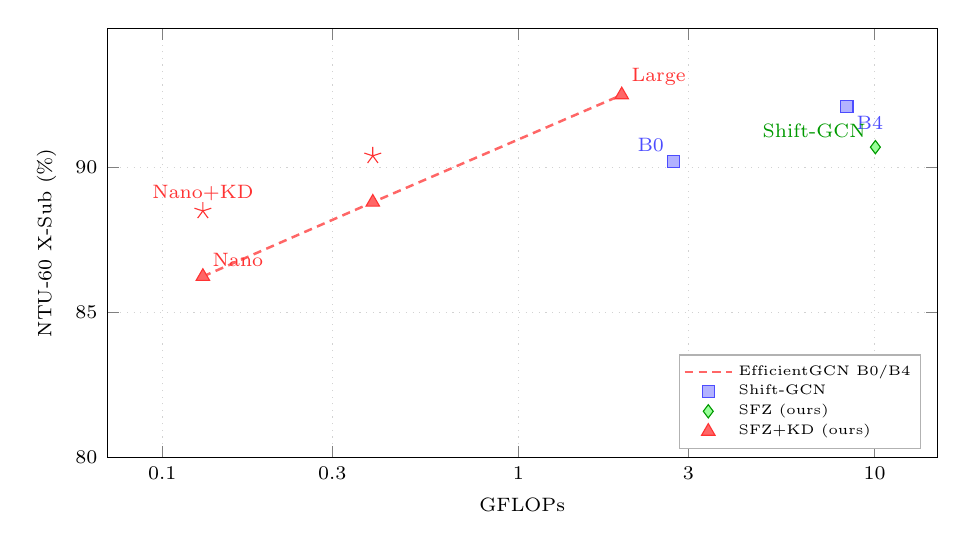
\begin{tikzpicture}
\begin{axis}[
  xmode=log,
  xlabel={GFLOPs},
  ylabel={NTU-60 X-Sub (\%)},
  xmin=0.07, xmax=15,
  ymin=80.0, ymax=94.8,
  xtick={0.1,0.3,1,3,10},
  xticklabels={0.1,0.3,1,3,10},
  minor xtick={},
  width=\columnwidth,
  height=0.58\columnwidth,
  grid=major,
  grid style={dotted,gray!35},
  tick label style={font=\scriptsize},
  label style={font=\scriptsize},
  legend style={font=\tiny, at={(0.98,0.02)}, anchor=south east,
                cells={anchor=west}, draw=gray!60,
                inner sep=1.5pt, row sep=-2pt},
  clip=true,
]

%% ── Pareto frontier (primary no-KD results only) ────────────────────────────
\addplot[densely dashed, color=red!60, line width=0.9pt] coordinates {
  (0.13,86.24)(0.39,88.8)(1.95,92.5)
};

%% ── EfficientGCN (blue squares) ─────────────────────────────────────────────
\addplot[only marks, mark=square*, mark size=2.2pt,
         draw=blue!70, fill=blue!30]
  coordinates { (2.73,90.2)(8.36,92.1) };
\addlegendentry{EfficientGCN B0/B4};

%% ── Shift-GCN (green diamond) ───────────────────────────────────────────────
\addplot[only marks, mark=diamond*, mark size=2.4pt,
         draw=green!60!black, fill=green!40]
  coordinates { (10.05,90.7) };
\addlegendentry{Shift-GCN};

%% ── SFZ no-KD (solid red triangles) ────────────────────────────────────────
\addplot[only marks, mark=triangle*, mark size=2.8pt,
         draw=red!80, fill=red!60]
  coordinates { (0.13,86.24)(0.39,88.8)(1.95,92.5) };
\addlegendentry{SFZ (ours)};

%% ── SFZ + KD (red stars) ────────────────────────────────────────────────────
\addplot[only marks, mark=star, mark size=3.2pt,
         draw=red!80, fill=red!80]
  coordinates { (0.13,88.5)(0.39,90.4) };
\addlegendentry{SFZ+KD (ours)};

%% ── Labels ───────────────────────────────────────────────────────────────────
\node[font=\scriptsize, text=red!80, anchor=south west]
  at (axis cs:0.13,86.24) {Nano};
\node[font=\scriptsize, text=red!80, anchor=south]
  at (axis cs:0.13,88.5)  {Nano+KD};
\node[font=\scriptsize, text=red!80, anchor=south west]
  at (axis cs:1.95,92.5)   {Large};
\node[font=\scriptsize, text=blue!70, anchor=south east]
  at (axis cs:2.73,90.2)  {B0};
\node[font=\scriptsize, text=blue!70, anchor=north west]
  at (axis cs:8.36,92.1)   {B4};
\node[font=\scriptsize, text=green!60!black, anchor=south east]
  at (axis cs:10.05,90.7)  {Shift-GCN};

\end{axis}
\end{tikzpicture}
